%% pairwise_genome_alignment.tex
%% Author: Leighton Pritchard
%% Copyright: James Hutton Institute
%% Pairwise genome alignment approaches

%
\begin{frame}
  \frametitle{Pairwise genome alignments}
  \textcolor{olive}{Genome sequence data gives us much more detail and power} \\
  Pairwise comparisons require alignment of similar regions.
  \begin{center}
    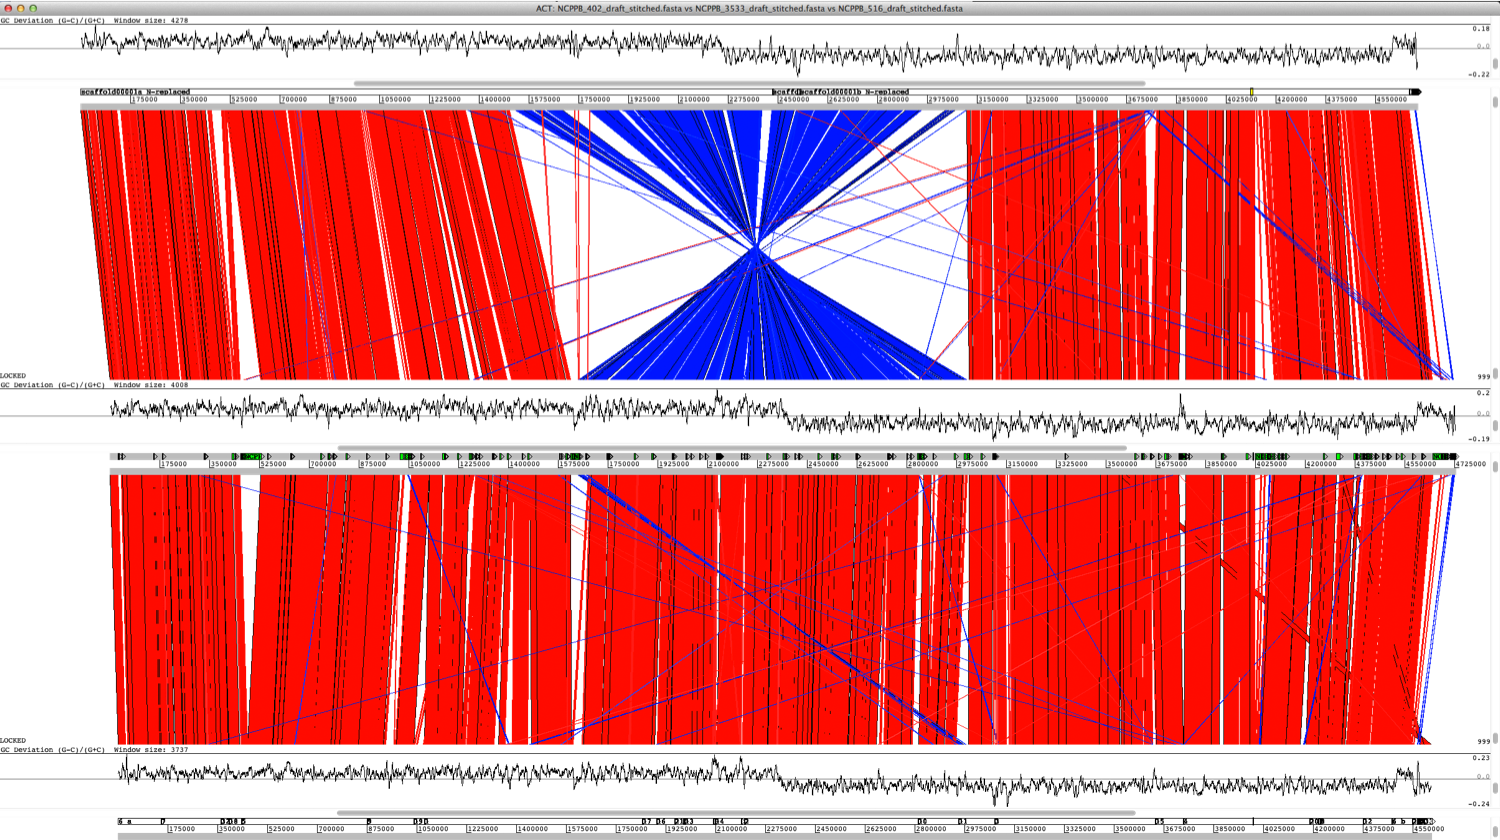
\includegraphics[width=\textwidth]{images/pairwise_genome_alignment}
  \end{center}  
\end{frame}

%
\begin{frame}
  \frametitle{Pairwise genome alignments}
  \textcolor{hutton_green}{Which genomes should you align (or not bother with)?} \\
  \textcolor{RawSienna}{For reasonable analysis, genomes should}:
  \begin{itemize}
    \item derive from a sufficiently \textcolor{red}{recent} common ancestor, so that \textcolor{hutton_purple}{homologous regions can be identified}
    \item derive from a sufficiently \textcolor{red}{distant} common ancestor, so that \textcolor{hutton_purple}{biologically meaningful changes are likely to be found}
  \end{itemize}
  \textcolor{hutton_blue}{They should also help answer your biological question}
  \begin{itemize}
    \item are you looking for organism, or phenotype-specific differences?
    \item are you investigating a process?
  \end{itemize}  
  This may be more involved for metazoans (vertebrates, arthropod, nematodes, etc.) than for prokaryotes
\end{frame}